\documentclass[12pt]{article}

\usepackage{pablo-devoir}
\usepackage[a5paper,margin=2cm]{geometry}

\pagestyle{empty}

\title{(In)Équations\\Corrigé}
\date{}
\classe{2\up{des}14}
\dsnum{DM 2}

\begin{document}

\maketitle
\begin{exercice}[Développement --- Factorisation]
  \emph{Soient les trois fonctions suivantes :}
  \begin{itemize}[$\bullet$]
    \item $f(x)=x^2-4x-5$
    \item $f_1(x)=\left( x+1 \right)\left( x-5 \right)$
    \item $f_2(x)=\left( x-2 \right)^2-9$
  \end{itemize}
  
  \begin{enumerate}
    \item \emph{Montrer que les trois formes $f$, $f_1$ et $f_2$ sont égales.}

      Commençons par développer $f_1$:
      \begin{align*}
        f_1(x) &= x\times x+x\times(-5)+1\times x+1\times(-5)\\
               &= x^2-5x+x-5\\
               &= x^2-4x-5\\
               &=f(x)
      \end{align*}
      Donc $f_1$ et $f$ sont égales. De même, pour $f_2$ et $f$ :
      \begin{align*}
        f_2(x) &= x^2-2\times2x+4-9\\
               &= x^2-4x-5\\
               &= f(x)
      \end{align*}
      Donc $f_2$ et $f$ sont égales. Les trois formes sont donc égales.
    \item \emph{Calculer $f(0)$ et $f(5)$.}
      Pour ces calculs, n'importe laquelle de ces formes convient, même si les calculs peuvent être plus simples avec l'une qu'avec l'autre.

      \begin{align*}
        f(0) &= 0^2-4\times0-5\\
             &= -5
      \end{align*}

      \begin{align*}
        f(5) &= 5^2-4\times5-5\\
             &= 25-20-5\\
             &= 0
      \end{align*}

    \item \emph{En utilisant la forme appropriée, résoudre les équations suivantes :}

      \begin{enumerate}[(a)]
        \item $f(x)=0$ :
          Nous utilisons ici la forme $f_1$ :
            $\left( x+1 \right)\left( x-5 \right) = 0$.
          C'est une équation produit, donc $x+1=0$ ou $x-5=0$, et donc $x=-1$ ou $x=5$.

        \item $f(x)=-9$ : Nous utilisons ici la forme $f_2$ : $\left( x-2 \right)^2-9=-9$. Donc $\left( x-2 \right)^2=0$. Puisque 0 est le seul nombre dont le carré vaut 0, cela donne $x-2=0$, et $x=2$. L'équation a une unique solution 2.
        \item $f(x)=-5$ : Nous utilisons la forme $f$ :
          \begin{align*}
            x^2-4x-5 &= -5\\
            x^2-4x&=0\\
            x\left( x-4 \right)&=0
          \end{align*}
          C'est une équation produit : $x=0$ ou $x-4=0$. Donc il y a deux solutions : 0 et 4.
      \end{enumerate}
  \end{enumerate}
\end{exercice}

\pagebreak

\begin{exercice}[Inéquations]
  \emph{Résoudre les inéquations suivantes, et présenter le résultat sous forme d'intervalles.}
  \begin{enumerate}[(a)]
    \item 
      \begin{multicols}{2}
      \begin{align*}
        4x-7 &\leq 10x+8\\
        -7-8 &\leq10x-4x\\
        -15 &\leq6x\\
        -\frac{15}{6} &\leq x\\
        -\frac{5}{2} &\leq x
      \end{align*}

      Représentée sur la droite des réels, cela donne :

      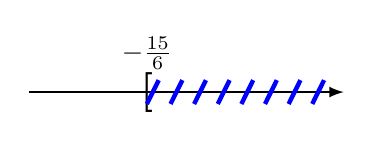
\begin{tikzpicture}[thick]
        \draw[-latex] (-4,0) -- (0,0);
        \draw ( {-5/2},0) node{{\Large\textbf{[}}} node[above=1ex]{$-\frac{15}{6}$};
        \foreach \i in {-2.5, -2.2, ..., -.3} {
          \draw[blue, ultra thick] (\i,-1ex) -- ({\i+.15},1ex);
        }
      \end{tikzpicture}
      \end{multicols}

      Et l'intervalle des solutions est donc $x\in\left[ -\frac{5}{2};+\infty \right[$.
    \item 
      \begin{multicols}{2}
      \begin{align*}
        9+3x&<-2\\
        3x&<-2-9\\
        3x&<-11\\
        x&<-\frac{11}{3}
      \end{align*}

      Représentée sur la droite des réels, cela donne :

      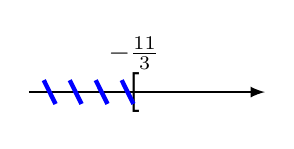
\begin{tikzpicture}[thick]
        \draw[-latex] (-5,0) -- (-2,0);
        \draw ( {-11/3},0) node{{\Large\textbf{[}}} node[above=1ex]{$-\frac{11}{3}$};
        \foreach \i in {-3.67, -4, ..., -4.8} {
          \draw[blue, ultra thick] (\i,-1ex) -- ({\i-.15},1ex);
        }
      \end{tikzpicture}
    \end{multicols}

      Et l'intervalle des solutions est donc $x\in\left] -\infty; -\frac{11}{3}\right[$.
    \item 
      \[
        \begin{array}{rl@{\text{ et }}rl}
        1+x & <2 & x+3 & \geq 0\\
        x & <2-1 & x & \geq 0-3\\
        x & <1 & x & \geq -3\\
      \end{array}
    \]

      Représentée sur la droite des réels, cela donne :

      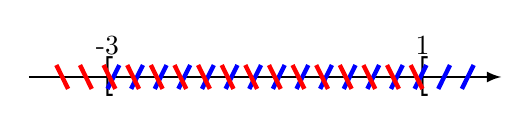
\begin{tikzpicture}[thick]
        \draw[-latex] (-4,0) -- (2,0);
        \draw ( -3,0) node{{\Large\textbf{[}}} node[above=1ex]{-3};
        \draw ( 1,0) node{{\Large\textbf{[}}} node[above=1ex]{1};
        \foreach \i in {-3, -2.7, ..., 1.8} {
          \draw[blue, ultra thick] (\i,-1ex) -- ({\i+.15},1ex);
        }
        \foreach \i in {1, .7, ..., -3.8} {
          \draw[red, ultra thick] (\i,-1ex) -- ({\i-.15},1ex);
        }
      \end{tikzpicture}

      Et l'intervalle des solutions est donc $x\in\left[ -3;1 \right[$.
    \item 
      \begin{align*}
        2\left( x+1 \right)&<-1+2x\\
        2 x+2 &<-1+2x\\
        2 x-2x &<-1-2\\
        0&<-3
      \end{align*}

    Cette dernière équation est toujours fausse, donc cette inéquation n'a pas de solutions. Cela peut être traduit par $x\in\emptyset$.
  \end{enumerate}
\end{exercice}


\begin{exercice}[Problème ouvert]~
  \begin{multicols}{2}
    \emph{Pour quelles valeurs de $x$ est-il possible de construire le triangle ci-contre ?}

  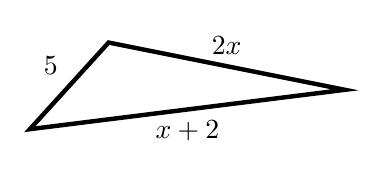
\begin{tikzpicture}[ultra thick]
    \draw (0,-0.4) -- (3,-1) node[midway,above]{$2x$} -- (-1,-1.5) node[midway,below]{$x+2$}-- cycle node[midway,above left]{$5$};
\end{tikzpicture}

\end{multicols}
Il est possible de construire un triangle si la longueur de chaque côté est inférieure ou égale à la somme des longueurs des deux autres côtés. Donc le nombre $x$ doit vérifier les trois inéquations suivantes.
\[\left\{\begin{array}{r@{\ \leq\ }l}
    5 & 2x+x+2\\
    2x & 5+x+2\\
    x+2 & 5+2x
\end{array}\right.\]

Une fois résolues, ces inéquations deviennent :

\[\left\{\begin{array}{r@{\ \leq\ }l}
    1 & x\\
    x & 7\\
    -3 & x
\end{array}\right.\]

La dernière inéquation est inutile (si, comme le montre la première inéquation, $1\leq x$, alors nécessairement $-3\leq x$), donc nous pouvons l'ignorer. Ainsi, $x$ vérifie : $1\leq x \leq7$, ou encore $x\in\left[ 1;7 \right]$. En d'autres termes, il est possible de construire un tel triangle si $x$ est compris entre 1 et 7.
\end{exercice}

\end{document}
